\documentclass{report}

\usepackage{eurosym}
\usepackage{hyperref}
\usepackage{biblatex}
\usepackage{graphicx}
\usepackage[T1]{fontenc}

\newcommand{\ignore}[1]{}

\addbibresource{refs.bib}
\graphicspath{{./img}}

\title{Manga-check}

\author{Blascovich Alessio\\
	\texttt{alessio.blascovich@studenti.unitn.it}
	\and
	Tomassi Jan\\
	\texttt{jan.tomassi@studenti.unitn.it}
}

\begin{document}

\maketitle

\tableofcontents

\newpage

\chapter{Introduzione}

La maggior parte delle applicazioni/piattaforme di lettura si basa su un
modello ad abbonamento, un utente pagando una quota mensile può leggere
tutto il catalogo dei manga della piattaforma.

Il problema di queste applicazioni è che vincola l'utente a dover pagare
un abbonamento per poter leggere manga che potrebbe già possedere in
formato virtuale.

Le piattaforme/applicazioni per la catalogazione delle letture sono per
lo più gratis, ma permettono solo di gestire le proprie letture senza
alcuna forma di reader in app.

La nostra idea è quella di colmare questa fascia di mercato,
\textbf{Manga-check} sarà questo il nome, dovrà permettere all'utente di
leggere qualsiasi manga lui possegga (formato \emph{.cbz}) e tramite una GUI
dare la possibilità di catalogare le proprie letture.

L'utente avrò anche la possibilità di eseguire un log-in per mantenere
la propria lista delle letture su più dispositivi.

L'applicazione darà la possibilità di leggere sia manga che sono nella
memoria del dispositivo che si sta utilizzando, ma anche di leggere da
un server ftp remoto del quale l'utente possiede le credenziali.

\section{Stack tecnologico}
\begin{itemize}
	\item Version control: git
	\item Online repository: github
	\item Editor: Android Studio
	\item Language: Kotlin
	\item Design style: Material
	\item DBMS: sqllite o PostgresSQL
\end{itemize}

\chapter{Identificazione del segmento utente}

In Europa, come nel resto del mondo, il mercato dei lettori di manga è
in costante aumento~\cite{mangaOut}.

Pur ampliandosi a fasce d'età superiori, il mercato dei Manga rimane
molto legato ad un pubblico giovane che preferisce il formato digitale.

Il formato digitale viene preferito per una serie di ragioni:

\begin{itemize}
	\item Costi inferiori rispetto alle coppie fisiche, un volume standard costa almeno \euro{5}
	\item Tempi di attesa di per ricevere volume/capitolo
	\item Reperibilità da un catalogo vastissimo
	\item Facilita un primo approccio ad una nuova serie
\end{itemize}

Per una velocità della lettura e portabilità la maggior parte degli
utenti preferisce leggere i propri Manga su un dispositivo mobile~\cite{NLTreport}

Per i motivi sopra citati la fascia d'età che potrebbe godere
maggiormente della nostra applicazione sono i ragazzi/rgazze tra i 12 ed
i 18 anni ed i giovani adulti tra i 19 e 25 anni.

\chapter{Stato dell'arte}

Le principali applicazioni per la lettura di manga sono 3 ma si basano
tutte su un abbonamento mensile e lettura solo online.

\begin{itemize}
	\item
	      \section{MangaToon} con più di 10 milioni di download e una media di 3.8 stelle su 5.\\
	      L'applicazione è parzialmente gratuita ma manca di alcune traduzioni, una ritardo nella pubblicazione settimanale dei capitoli e nessuna possibilità di mantenere una lista delle letture.\\
	      Il catalogo è basato solo su Manga prodotti da case indipendenti.\\
	      L'app è monotematica per quanto riguarda la demografia delle letture, tutti i titoli sono Shojo~\cite{shooManga}.\\
	      Gli utenti lamentano troppe limitazioni nella versione gratuita e delle pubblicità troppo invasive.\\
	      Link per la pagina del Play Store.
	\item
	      \section{MANGA Plus}con più di 10 milioni di download e una media di 4.1 stelle su 5.\\
	      L'app parte da un abbonamento gratis che permette di leggere una parte molto ridotta del catalogo.\\
	      Essendo un'applicazione di origine orientale la UI risulta molto diversa dai canoni occidentali, con elementi che distraggono l'occhio e immagini molto grandi e piene di elementi.\\
	      Apparentemente non è possibile effettuare un log in per sincronizzare tra i vari dispositivi l'elenco delle letture.\\
	      Presenta anche una sezione dove gli autori più piccoli possono pubblicare i loro lavori in modo facilitato.\\
	      Link per la pagina dal Play Store.
	\item
	      \section{Crunchyroll Manga} con più di 5 milioni di download e una media di 2.8 stelle su 5.\\
	      L'applicazione presenta un abbonamento gratis ed uno premium, con l'abbonamento gratis si ha accesso solo al primo capitolo di alcune opere il che inficia molto sull'esperienza dell'utente.\\
	      A dispetto degli screen sul play store molte opere di grande rilievo non sono presenti e si possono leggere solo Manga indipendenti.\\
	      La UI risulta molto facile da navigare e pulita, anche il reader è molto facile da usare e tiene traccia della pagina alla quale si è arrivati.\\
	      Link per la pagina del Play Store.
\end{itemize}

La nostra applicazione, come detto, si mette in contrapposizione a
questa corrente di mercato fornendo un prodotto gratis ma che si basa
sulla lettura offline.\\
L'utente anziché pagare un abbonamento mensile potrebbe acquistare i
Manga in formato digitale e leggerli sulla nostra applicazione.\\
L'incentivo ad usare la nostra applicazione è dato dalla possibilità di
gestire le proprie letture in modo simile a come fa la piattaforma
online.

All'utente viene quindi tolta la difficoltà di dover navigare attraverso
due applicazioni separate per reader e manager.

\chapter{Wireframe e navigazione}

\section{Digressione Material Design}

Le interfacce grafiche dell'applicazione sono state realizzate seguendo il più possibile gli standard imposti da Material Design 3~\cite{matDes}.\\
In alcuni casi come nella ricerca dell'indice all'interno del \hyperref[sec:raeder]{Reader} abbiamo preferito divergere delle linee guida di Material Design 3 per una UX migliore da parte dell'utente.

\section{Library \- Home page}\label{sec:home}

\begin{center}
   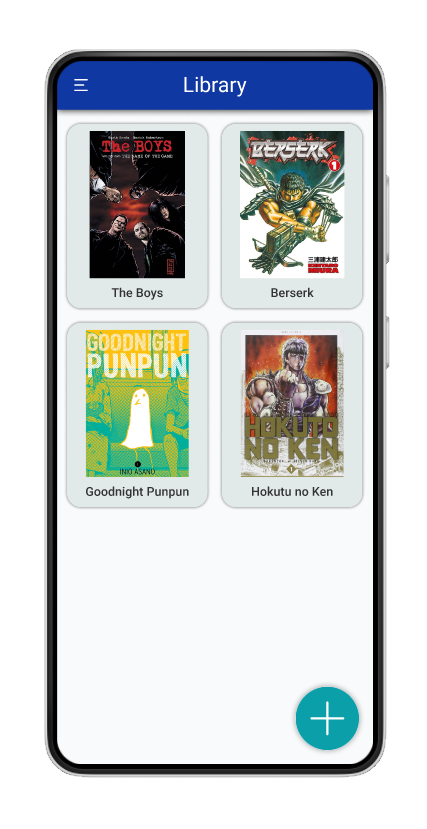
\includegraphics[scale=0.4]{library_home_page.png}
\end{center}

L'applicazione si avvierà nella schermata contenente la libreria del lettore.\\
La libreria presenterà le opere possedute dall'utente ognuna contrassegnata dal nome .\\
Cliccando sull'anteprima di uno dei fumetti verrà aperta la \hyperref[sec:comic_list]{Comic List}, mentre premendo sull'icona nell'angolo superiore sinistro verrà aperto un \hyperref[sec:hamburger]{Menù ad hamburger}.\\
Nell'angolo in basso a destra sarà presente un bottone per aggiungere una nuova opera le cui informazioni verranno recuperate dal database remoto che fa da supporto all'applicazione, le informazioni recuperate saranno titolo, immagine di anteprima, breve descrizione, $\dots$\\
La ricerca nel database verrà effettuata tramite il fragment \hyperref[sec:add_library]{Add Library}
Se invece si vuole aggiungere un nuovo capitolo/volume bisognerà entrare nell'opera di appartenenze e selezionare dai file locali o dal server FTP il capitolo/volume che vogliamo aggiungere.

\section{Comic List}\label{sec:comic_list}

\begin{center}
  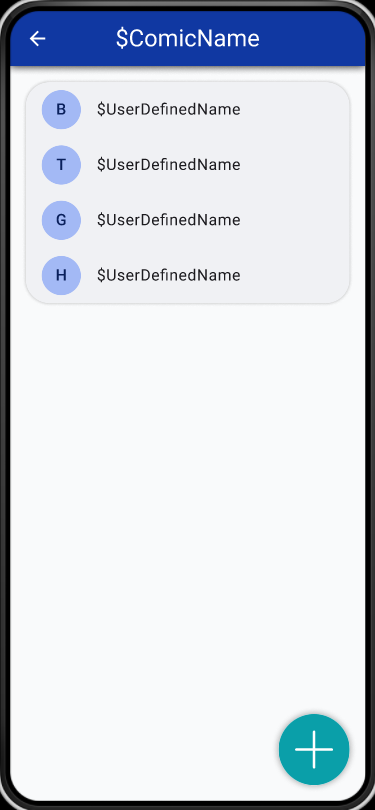
\includegraphics[scale=0.4]{comic_list.png}
\end{center}

In questa schermata l'utente troverà la lista dei volumi/capitoli, di un'opera, che ha caricato all'interno dell'applicazione.\\
Con il tasto ``+'' posizionato nell'angolo inferiore destro potrà aggiungere un nuovo capitolo/volume associato all'opera, mentre tenendo premuto premuto sul nome di un elemento della lista potrà aggiornarne gli attributi tramite il form presente in \hyperref[sec:update_comic]{Update Comic}.\\
Infine premendo su un volume/capitolo si verrà portati al \hyperref[sec:reader]{Reader}.

\section{File Manager}

\begin{center}
  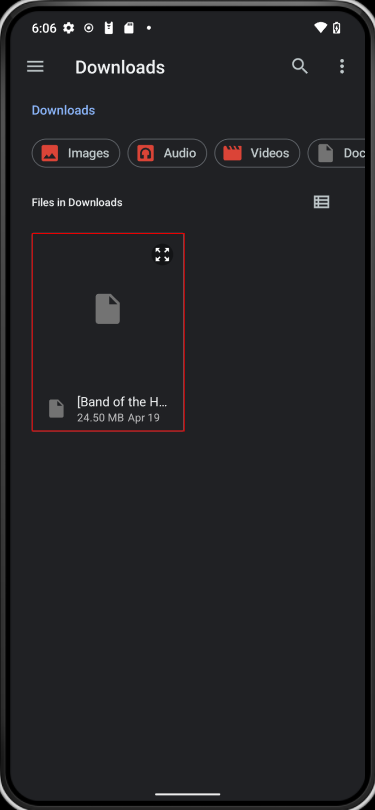
\includegraphics[scale=0.4]{file_manager.png}
\end{center}

L'applicazioen dovrà interfacciarsi con il file manager per poter permettere all'utente di selezionare i file \emph{.cbz} da caricare.\\
Una volta selezionato il file si verrà portati nel fragment \hyperref[sec:add_chapter]{Add chapter}.

\section{Add Chapter}\label{sec:add_chapter}

\begin{center}
  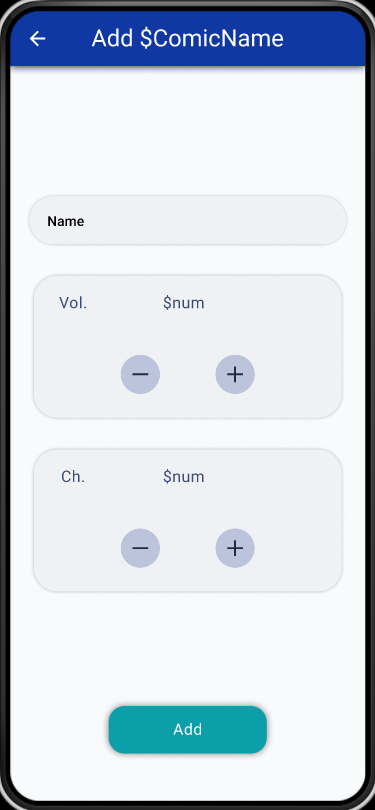
\includegraphics[scale=0.4]{add_chapter.png}
\end{center}

Tramite un breve form l'utente potrà modificare il nome del file e indicare che capitolo sta inserendo.\\
Il capitolo indicato dall'utente non andrà in alcun modo a modificare i contenuti della \hyperref[sec:reading_list]{Reading List} ma serìvirà solo a mantenere una numerazione all'interno della vista \hyperref[sec:comic_list]{Comic List}.

\section{Update Comic}\label{sec:update_comic}

\begin{center}
  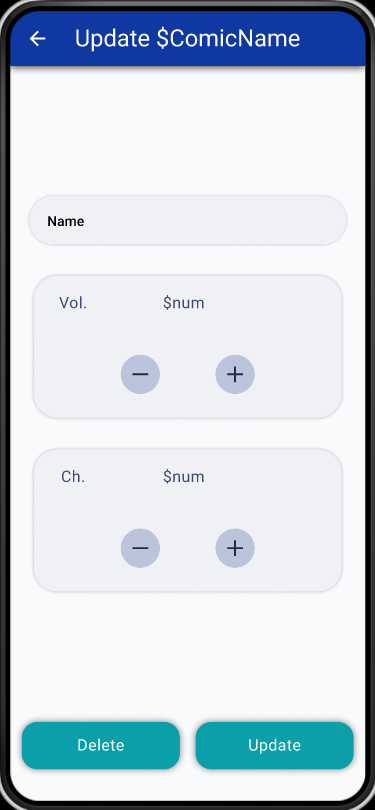
\includegraphics[scale=0.4]{update_library.png}
\end{center}

Tramite un form simile a \hyperref[sec:add_chapter]{Add Chapter} l'utente potrà andare a modificare i dati con cui è stato salvato il capitolo/volume dell'opera selezionata.

\section{Add Library}\label{sec:add_library}

\begin{center}
  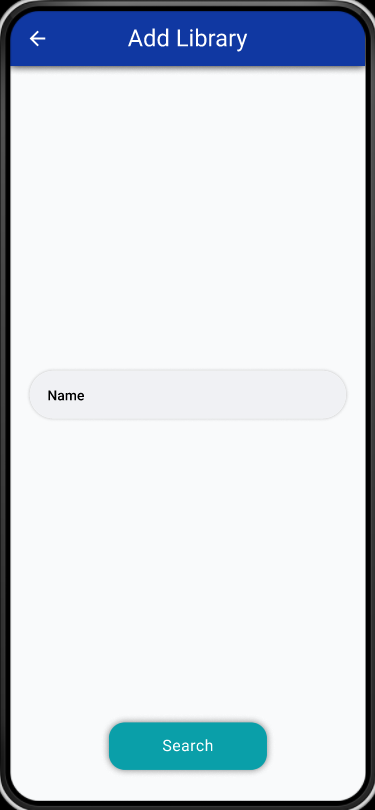
\includegraphics[scale=0.4]{add_library.png}
\end{center}

Tramite una casella di testo l'utente potrà interrogare il database remoto così d aggiungere in locale una nuova opera con le relative informazioni.

\section{Reader}\label{sec:reader}

\begin{center}
   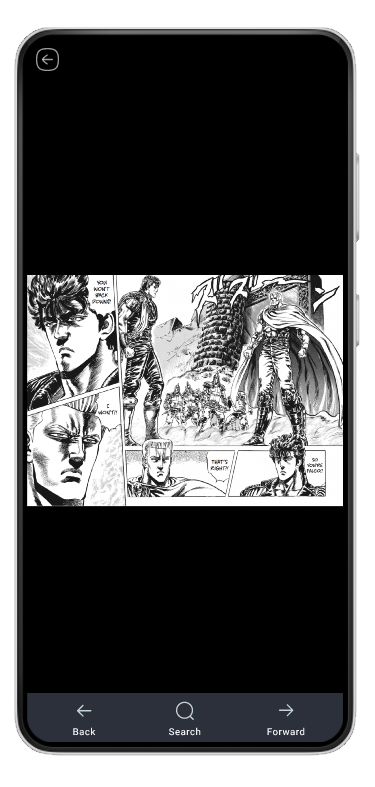
\includegraphics[scale=0.4]{reader.png}   
\end{center}

La schermata del Reader conterrà una barra di navigazione nel lato inferiore dello schermo.\\
La barra di navigazione avrà dei comandi basici per moversi all'interno del file, un bottone per andare alla pagina precedente, uno per andare a quella successiva e uno per ricercare la pagina con un determinato numero.\\
Il numero con cui si effettuerà la ricerca sarà assoluto e.g.\ la copertina sarà la pagina numero 1.\\
Nella parte superiore dello schermo sarà presente una freccia per poter tornare alla \ignore{\hyperref[sec:home]{Library \- Home page}} schermata dell'opera e interrompere la lettura.

\section{Search dialog}

\begin{center}
   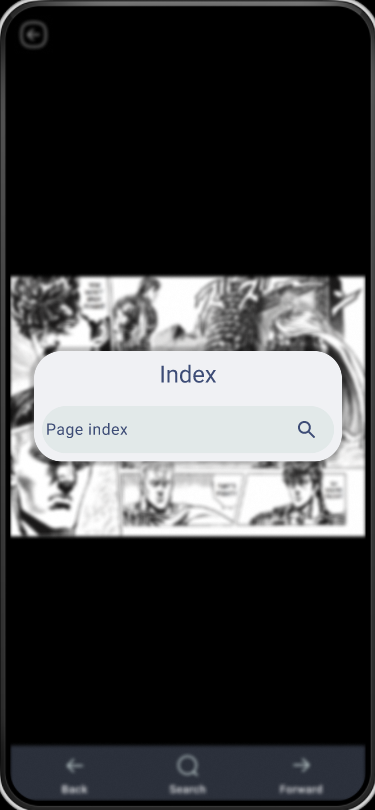
\includegraphics[scale=0.4]{search_dialog.png}
\end{center}

Una volta premuto sull'icona della ricerca vierrà aperto un dialog dove verrà chiesto all'utente di inserire l'indice della pagina alla quale si vuole andare.\\
Il formato di file scelto, ovvero \emph{.cbz}, non contiene metadati per l'enumerazione, quindi la numerazione inizia con la prima schermata che avrà indice 1.\\
Questa potrebbe essere una debolezza ma ogni altro lettore di \emph{.cbz} contiene questa imperfezione.

\section{Menù ad hamburger}\label{sec:hamburger}

\begin{center}
   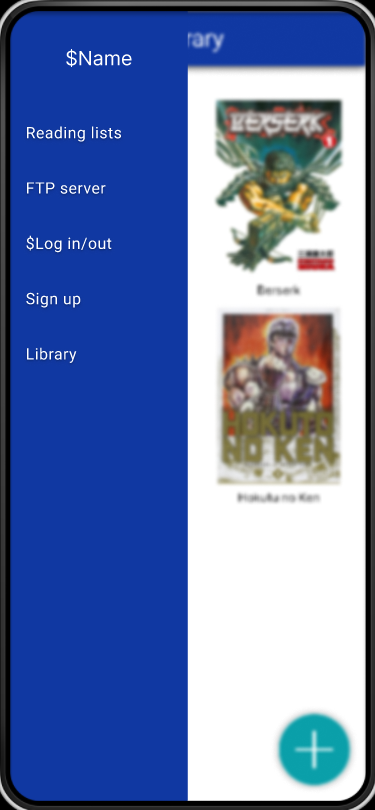
\includegraphics[scale=0.4]{hamburger.png}
\end{center}

Il Menù ad hamburger conterrà lo user name se l'utente ha effettuato il log in, altrimenti lascerà uno spazio vuoto.\\
Il resto del menù conterrà una lista con le seguenti voci:
\begin{itemize}
   \item \textbf{Reading list} che porterà l'utente alla propria lista delle letture.
   \item \textbf{FTP server} permetterà all'utente di configurare il proprio server FTP dal quale dopo scaricare materiale.
   \item \textbf{Log in/out} sarà una stringa adattiva, se l'utente non è loggato presenterà la scritta ``Log In'' altrimenti la scritta ``Log Out''.
  \item \textbf{Sign Up} permetterà all'utente di registrare un nuovo profilo, sarà presente solo se l'utente deve ancora effettuare l'accesso.
  \item \textbf{Library} creerà una shortcut per poter tornare alla \hyperref[sec:home]{Library \- Home page}.
\end{itemize}

\section{Reading list}\label{sec:reading_list}

\begin{center}
   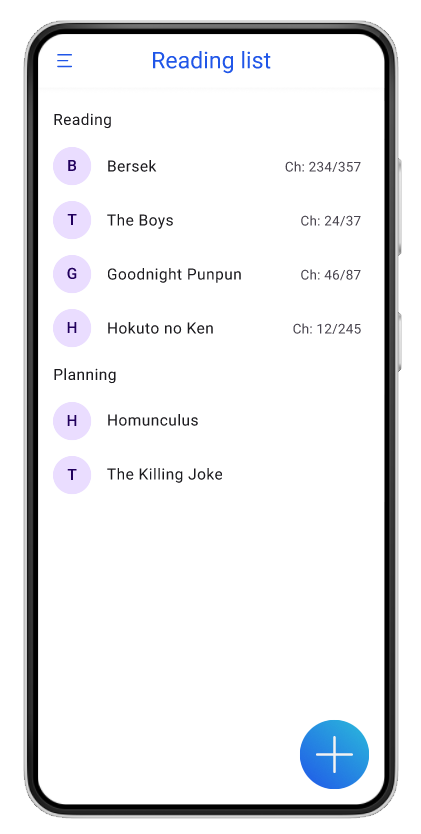
\includegraphics[scale=0.4]{reading_list.png}
\end{center}

La reading list conterrà una lista delle letture che sono state inserite dall'utente.\\
Queste letture saranno divise in più categorie:
\begin{itemize}
   \item \textbf{Reading} conterrà le opere ch l'utente sta leggendo.\\
   In questa lista affiancato al nome dell'opere ci sarà un indicatore per modificare il capitolo al quale si è arrivati.
   \item \textbf{Planning} quelle che pianificherà di leggere in futuro.
   \item \textbf{Completed} le letture che l'utente ha concluso.
\end{itemize}
Premendo su un item della lista sarà possibile aggiornare il numero del capitolo, i reading avranno capitoli maggiori uguali a 1, i planninig avranno capitolo attuale uguale a 0 mentre i completed avranno capitolo uguale all'ultimo capitolo uscito.\\
Per rimuovere una lettura basterà fare uno swipe e verrà rimossa dall'elenco.\\
Nella parte destra associto ad ogni lettura nella sezione \textbf{Reading} sarà presente il numero del capitolo al quale il lettore è arrivato, questo numero dovrà essere incrementato o diminuito dal lettore stesso, la modifica avverrà tramite il dialog \hyperref[sec:info_reading]{Info reading}.

\section{Info reading}\label{sec:info_reading}

\begin{center}
   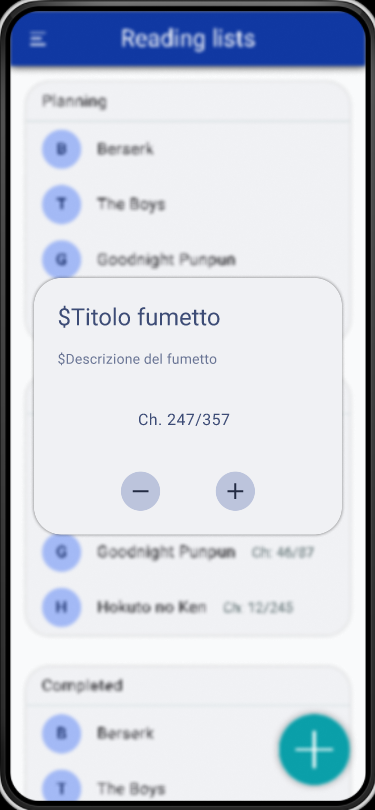
\includegraphics[scale=0.4]{info_reading.png}
\end{center}

Da questa finestra di dialog sarrà possibile incrementare o decrementare il numero dei capitoli letti di un'opera selezionata.\\
Sopra il selettore dei capitoli sarà presente il titoletto dell'opera e una breve descrizione di essa.\\
L'utente potrà accedere a questa finestra di dialog premendo sul titolo di un'opera.\\

\section{Add reading}

\begin{center}
   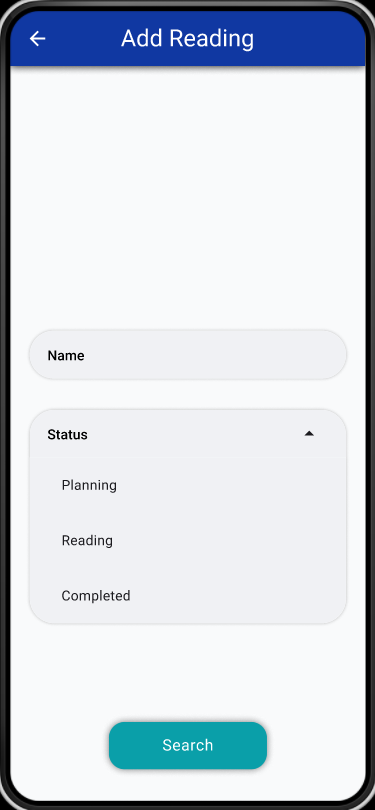
\includegraphics[scale=0.4]{add_reading.png}
\end{center}

Tramite questa interfaccia l'utente potrà aggiungere una nuova opera alla sua \hyperref[sec:reading_list]{Reading list} in una categoria a scelta tra:
\begin{itemize}
   \item \textbf{Planning}
   \item \textbf{Reading}
   \item \textbf{Completed}
\end{itemize}
Le opere che l'utente potrà selezionare saranno quelle presenti nel database remoto al quale l'applicazione fa riferimento.

\section{Sign Up}

\begin{center}
   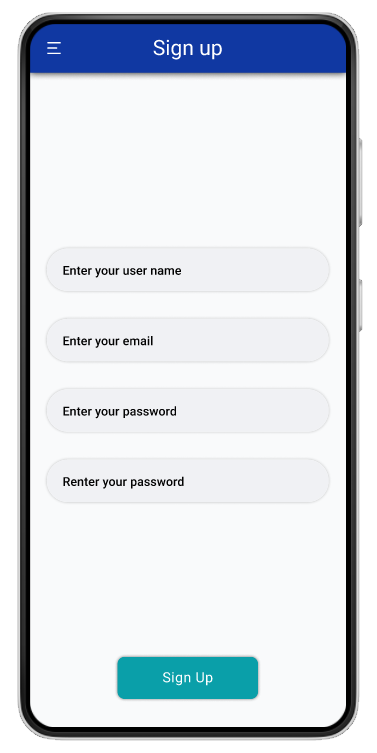
\includegraphics[scale=0.4]{sign_up.png}
\end{center}

Nel form per l'iscrizione al neo-utente verrà chiesto di inserire uno user name che verrà poi mostrato a schermo (nel \hyperref[sec:hamburger]{Menù ad hamburger}), una mail con la quale fare il log in e una password che dovrà essere inserita due volte.\\
Se uno dei parametri non rispetta ciò che il server aspetta il campo diventerà del colore assegnato agli errori e non si potrà proseguire con il log in.

\printbibliography

\end{document}
